\chapter{Game Development}
Aνάπτυξη βιντεοπαιχνιδιών (game development) ονομάζουμε τη διαδικασία της δημιουργίας ενός παιχνιδιού. Η ομάδα ανάπτυξης μπορεί να κυμαίνεται από ένα άτομο μέχρι μια μεγάλη επιχείρηση.			
	\section{Game Engineering}
	To game engineering περιλαμβάνει πολλές εξειδικευμένες ειδικότητες, οι οποίες παράγουν ένα game engine.
	\subsection{Game Engines}	
	Στο τομέα του σχεδιασμού παιχνιδιών το πιο διαδεδομένο CASE tool είναι η μηχανή γραφικών. Μια μηχανή γραφικών είναι μια σουίτα από επαναχρησιμοποιήσιμα οπτικά εργαλεία τα οποία βρίσκονται σε ένα ενιαίο περιβάλλον.
	Η κεντρική λειτουργικότητα η οποία παρέχεται περιλαμβάνει τη φωτοαπόδοση σε πραγματκό χρόνο (real time rendering) , τη μηχανή φυσικής και εντοπισμό συγκρούσεων (physics and collision detection), το scripting, το animation, την τεχνητή νοημοσύνη (Artificial Intelligence), τη δικτύωση (networking), τον παραλληλισμό ενεργειών (multitasking), την διαχείριση μνήμης και τον γράφο σκηνής (scene graph). Η ανάπτυξη τον παιχνιδιών μέσω μιας μηχανής γραφικών γίνεται εύκολα, γρήγορα και οδηγούμενη απο δεδομένα (data driven) ούτως ώστε οι δημιουργοί παιχνιδιών να μπορούν να ασχολούνται με τις λεπτομέρειες του παιχνιδιού τους.
	Οι μηχανές αναπτύσσονται από ομάδες που απαρτίζονται όχι μόνο από προγραμματιστές, αλλά και απο μαθηματικούς, φυσικούς κλπ. Η κάθε υπο-ομάδα εστιάζει σε ένα συγκεκριμένο κομμάτι, όπως οι φυσικοί με τον εντοπισμό συγκρούσεων, και αρχιτέκτονες λογισμικού σχεδιάζουν το πως τα κομμάτια συνδέονται και αλληλεπιδρούν μεταξύ τους, χωρίς να τους απασχολούν οι λεπτομέριες σχεδίασης του κάθε κομματιού.
	
	\subsection{Ιστορία}
	Η ιστορία των Βιντεοπαιχνιδιών, αρχίζει στα τέλη της δεκαετίας του '40. Προς τα τέλη του '50 και στα μέσα του '60, στην Αμερική, αρχίζουν να μπαίνουν στην καθημερινή μας ζωή, οι υπολογιστές. Για την ακρίβεια, οι κεντρικοί υπολογιστές. Από εκείνη την περίοδο, τα βιντεοπαιχνίδια έκαναν την εμφάνιση τους, στις κονσόλες, στα φλίπερ, στους υπολογιστές, αλλά και στις φορητές κονσόλες. Από τότε η δημιουργία παιχνιδιών έχει γιγαντιωθεί έχοντας ένα τεράστιο κομμάτι της παγκόσμιας οικονομίας.
	Πλέον ο ανταγωνισμός είναι τεράστιος, τα βιντεοπαιχνίδια κυκλοφορούν για διάφορες κονσόλες με  πολύ απαιτητικά γραφικά και με πολύ γρήγορο ρυθμό.
	\subsection {Τι είναι μια μηχανή γραφικών}
	Η πρώτη αναφορά σε μηχανή γραφικών έγινε στα μέσα της δεκαετίας του 90 και αναφερώταν στο δημοφιλές παιχνίδι Doom του οποίου η αρχιτεκτονική διαχώριζε τα βασικά συστήματα του παιχνιδιού, όπως rendering system, collision detection system, audio system, asset system κλπ. Η αξία αυτού του διαχωρισμού εκτιμήθηκε από την κοινότητα όταν οι προγραμματιστές ξεκίνησαν να πουλάνε άδειες για το λογισμικό, επαναχρησιμοποιούσαν εργαλεία προηγούμενων παιχνιδιών με δημιουργία νέων assets. Μικρότερα στούντιο τροποποιούσαν εκδόσεις υπάρχων παιχνιδιών χρησιμοποιωντας το SDK.ό
	Πολλά παιχνίδια γράφτηκαν με σκοπό να επαναχρησιμοποιηθούν κομμάτια κόδικα και modding. Πολλές μηχανές όπως η μηχανή του Quake III γράφτηκαν με τρόπο ώστε να είναι εύκολα προσαρμόσημες χρησιμοποιώντας scripting, με σκοπό την εμπορευματοποίηση μέσω licensing.
	Η διαχωριστική γραμμή μεταξύ του παιχνιδιού και της μηχανής δεν μπορεί να οριστεί με ακρίβεια. Πολλές μηχανές μπορεί να περιέχουν συγκεκριμένα μέρη που αφορούν συγκεκριμένη λειτουργία του παιχνιδιού. Η μεγάλη διαφορά είναι στο data-driven architecture όπου οι κανόνες και τα στοιχεία δεν είναι hard-coded αλλά διαβάζονται από εξωτερικό αρχείο.
	Οι μηχανές έχουν τα όριά τους ανάλογα με τα είδη παιχνιδιού στα οποία η μηχανή εστιάζει, σε ποιες πλατφόρμες, σε τι στιλ γραφικών, σε ποια αρχιτεκτονική της gpu κλπ. 
	
	\subsection{Γιατί μηχανές γραφικών;}	
	Η αφαίρεση πάντα βοηθούσε τον εγκέφαλο να λειτουργήσει καλύτερα και να κατανοήσει αλληλεπιδράσεις μεταξύ συστημάτων και περίπλοκες έννοιες. Οι μηχανές γραφικών απαλλάζουν τους γραφίστες και τους προγραμματιστές από τις τεχνικές λεπτομέριες, και εστιάζουν στην αισθητική και στο gameplay. Επίσης με την αποσύνδεση των συστημάτων έχουμε πιο προβλέψημη συμπεριφορά, επεκταστημότητα των υποσυστημάτων ως υποσυστήματα και ευκολη δοκιμαστικότητα.
	
\subsection{Δομή μιας μηχανής γραφικών}
Η μοντέλοποίηση της δομής των μηχανων γραφικών σε αφαιρετικό επίπεδο είναι πανομοιότυπη, διαφέρει όμως η υλοποίηση. Η δομή ξεκινά να διαφοροποιείται στα υψηλότερα επίπεδα, τα οποία υλοποιούνται με στόχο για σχεδιασμό συγκεκριμένου είδους παιχνιδιών. Μια τυπική μηχανή γραφικών παρουσιάζεται στο \ref{fig:Game_Engine_Architecture} \cite{gregory2009game}.
	\begin{figure}
		\centering
		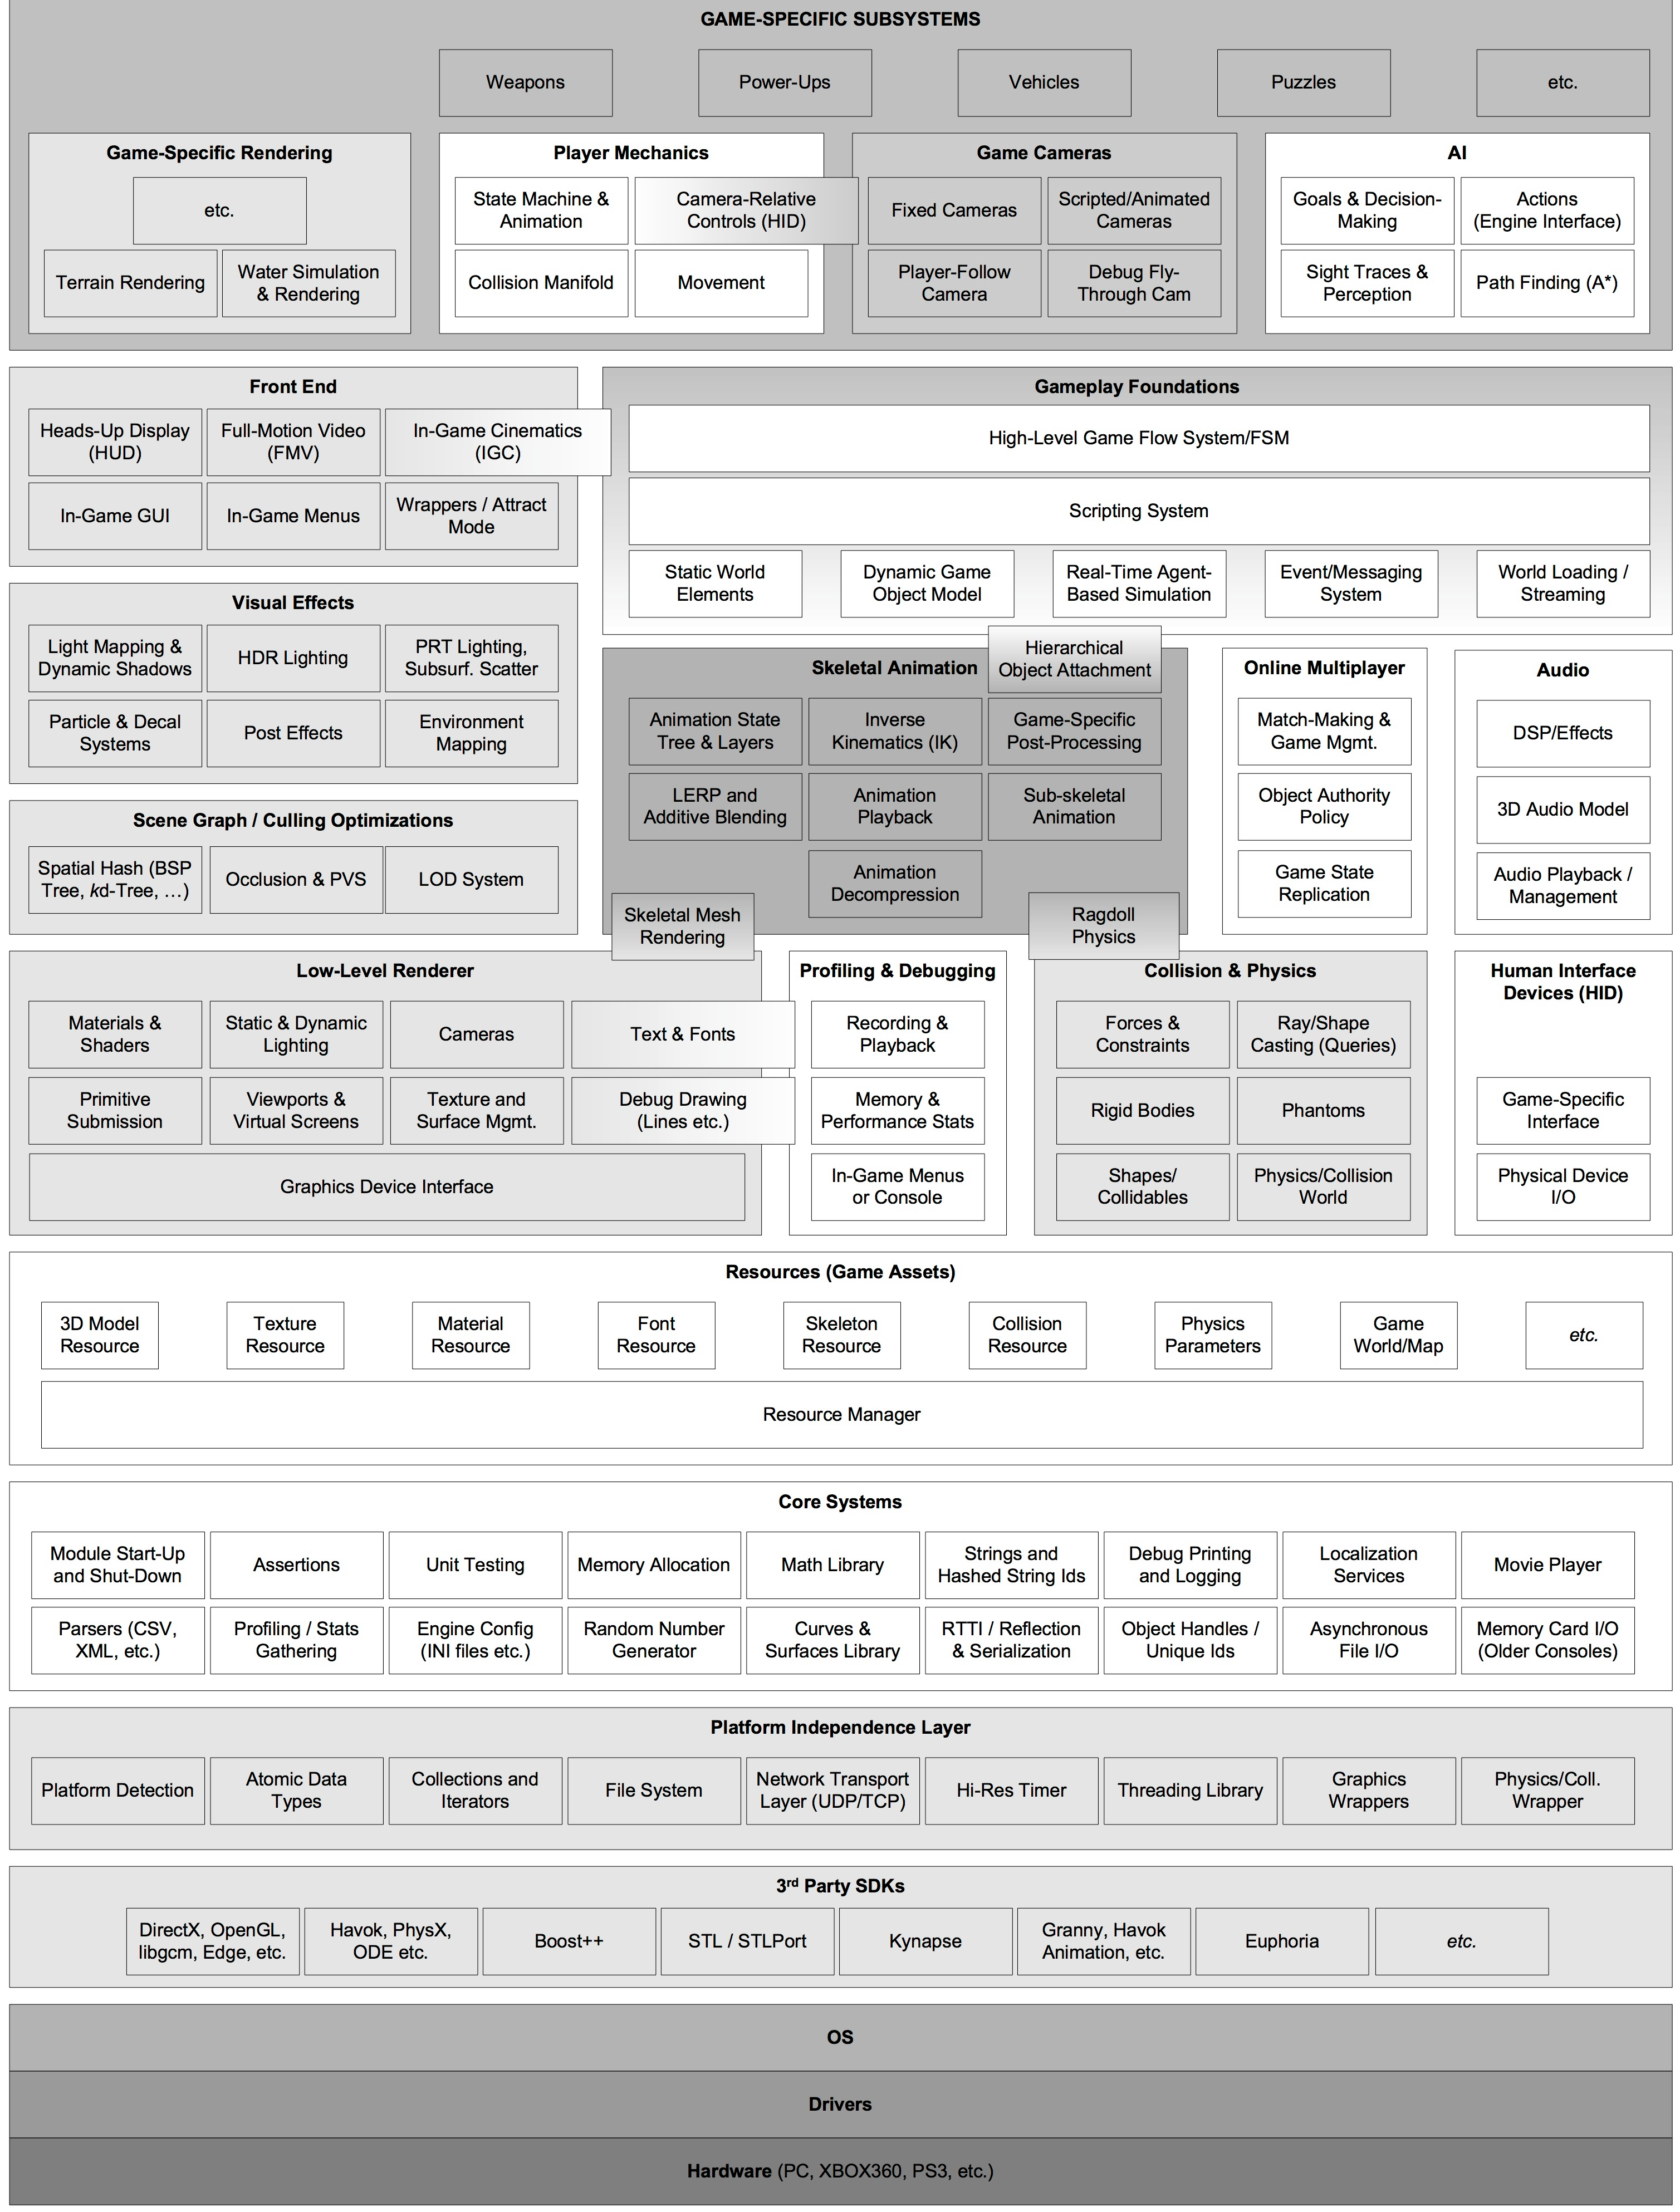
\includegraphics[width=160mm]{Images/game_engine_architecture}
		\caption{Τυπική αρχιτεκτονική μηχανής γραφικών}
		\label{fig:Game_Engine_Architecture}
	\end{figure}	

\paragraph{Επισκόπηση επιπέδων}
\begin{itemize}
\item
Hardware
Το hardware αντιπροσωπεύει το υλικό, δηλαδή το υπολογιστή ή κονσόλα στο οποίο θα τρέξει το παιχνίδι.
\item
Drivers
Τα drivers διαχειρίζονται τους πόρους του υλικού και του λειτουργικού ένα καθολικό προτόκολο επικοινωνίας μεταξύ των πολλών παραλλαγών.
\item
OS (Operating System)
Το λειτουργικό σύστημα είναι ο ενορχηστρωτής των προγραμμάτων. Κατανέμει το χρόνο μεταξύ των πόρων του υλικού και τον προγραμμάτων και παραλληλίζει την εκτέλεση προγραμμάτων. Στις κονσόλες το λειτουργικό παίζει τυπικό ρόλο, αφού το λογισμικό (παιχνίδια) έχουν σχεδόν πλήρη έλεγχο του υλικού. Πλέον όμως στις σύγχρονες κονσόλες και στα λειτουργικά συστήματα όπως Microsoft Windows, κανένα πρόγραμμα δεν έχει πλήρη έλεγχο, αφού το λειτουργικό μπορεί να μοιραστεί πόρους του συστήματος με το τρέχον λογισμικό για να εμφανίσει για παράδειγμα κάποιο μήνυμα.

\item
Third party SDKs and MiddleWare
Πολλές φορές χρησιμοποιούνται βιβλιοθήκες ανάπτυξης λογισμικού τρίτων, οι οποίες γράφτηκαν από την κοινότητα και λύνουν κοινά προβλήματα. Συχνό παράδειγμα είναι η χρήση βιβλιοθηκών για κοινές δομές δεδομένων, η για rendering.

\item
Collision and Physics
Εντοπισμός συγκρούσεων και rigid-body dynamics (physics) δηλαδή πως ένα σύστημα με διασυνδεδεμένα σώματα αντιδρά όταν του ασκούνται εξωτερικές δυνάμεις.

\item
Platform Independence Layer
Πολλά παιχνίδια καλούνται να τρέξουν σε περισσότερες από μία πλατφόρμες. Σε αυτό το επίπεδο ενθυλακώνονται οι εντολές στο λειτουργικό σύστημα και στο υλικό για να μπορούν να αλλάξουν ανάλογα με το περιβάλλον ανάπτυξης.

\item
Core Systems
Κάθε μεγάλο και σύνθετο πρόγραμμα χρειάζεται κάποιες γενικής χρήσης βιβλιοθήκες. Κάποιες από αυτές είναι: 

	\begin{itemize}
	\item Assertions
	 κώδικας ο οποίος ελέγχει υποθέσεις του προγραμματιστή για το πως θα τρέξει η συνάρτηση. Ο κώδικας αυτός αφαιρείται στις τελικές εκδόσεις, αφού περάσει η περίοδος δοκιμών.
	\item Memory Management: έλεγχος της μνήμης για αποφυγή fragmentation και out of memory.
	\item Βιβλιοθήκη μαθηματικών η οποία περιέχει μαθηματικά που εμφανίζονται στις προσομειώσεις πραγματικού χρόνου, όπως μαθηματικα διανυσμάτων, πινάκων, γεωμετριάς κλπ.
	\end{itemize}

\item Resource Management διαχείριση των πόρων του παιχνιδιού, όπως τα μοντέλα, τα textures, ο κόσμος, οι χάρτες κλπ
\item Rendering Engine το πιο σύνθετο κομμάτι, το οποίο είναι υπεύθυνο για την αναπαράσταση του παιχνιδιού στην οθόνη.
\item Low-level renderer  το οποίο εστιάζει στην βελτιστοποίηση των πρωτογενή γεωμετρικά σχήματα
που απαρτίζουν τα διάφορα κομμάτια.
\item Scene Graph η οποία καθορίζει ποια αντικείμενα πρέπει να γίνουν render από τη rendering engine χρησιμοποιώντας αλγόριθμους ανάλογα με το μέγεθος και το είδος του παιχνιδιού.
\item Visual Effects που αποτελούνται από particle systems, light mapping, dynamic shadows, anti-aliasin 
\item Front End πολλές φορές χρειάζεται κάποιο επίπεδο επικοινωνίας με το παιχνίδι, όπως μενού κονσόλα, pop-ups κλπ
\item Profiling and Debugging. Η ποιότητα της απόδοσης του παιχνιδιού είναι πολύ κρίσιμη. Για να γίνει βελτιστοποίηση της απόδοσης, χρειάζονται εργαλεία ανάλυσης του υλικού ενώ τρέχει το παιχνίδι με οπτική αναπαράσταση.
\item Collision and Physics
Η φυσική και οι συγκρούσεις είναι στενά συνδεδεμένες γιατί οι συγκρούσεις επιλυόνται με κανόνες φυσικής.
\item Animations
\item Human Interface Devices
Βιβλιοθήκες για έλεγχο των σημάτων από το πληκτρολόγιο, το ποντίκι, τα χειριστήρια τα οποία χρησιμοποιεί ο χρήστης για να επικοινωνήσει με το παιχνίδι. Επίσης πολλές φορές χρησιμοποιούνται για να επικοινωνήσει το παιχνίδι με το χρήστη, όπως η δόνηση στο χειριστήριο.
\item Audio
Το σύστημα διαχείρισης ήχου έχει πολλές δυνατότητες. Μπορεί να χρησιμοποιηθεί για τρισδιάστατη αναπαράσταση του ήχου, για να δώσει την αίσθηση του βάθους και της απόστασης στον χρήστη.
\item Online Multiplayer – Networking
Συνήθως ένας χρήστης παίζει μόνος του σε ένα εικονικό κόσμο. Πολλές φορές όμως άλλοι χρήστες συνδέονται σε αυτό τον κόσμο.
\item Gameplay Foundation Systems οι κανόνες του εικονικού κόσμου οι οποίοι οριοθετούν τις δυνατότητες του παίχτη
Game Worlds and Object Models
η αναπαράσταση του κόσμου με αντικειμενοστραφή τρόπο, το game object model.
Περιλαμβάνει το στατικό background, τα dynamic rigid bodies, τους παίχτες (Player Characters), τους non-player characters, τα όπλα, τα οχήματα, το φωτισμό, τις κάμερες κλπ.
\item Event System
το σύστημα που επιτρέπει την επικοινωνία μεταξύ του game object model.
\item Scripting System
To scripting σε μία μηχανή γραφικών, επιταχύνει την ανάπτυξη γιατί περιέχει χρήσιμες, συχνές και έτοιμες προς εκτελεση εντολές.
\item Artificial Intelligence
Τυπικά patterns νοημοσύνης, όπως navigation , path finding, dynamic object avoidance κλπ.
\item Game Specific Subsystems
Τα συστήματα που είναι χτισμένα πάνω από τη μηχανή γραφικών και αφορούν συγκεκριμένα το παιχνίδι.
\item Tools and Asset Pipeline
Όλα τα παιχνίδια χρειάζονται πολλά δεδομένα για να αναπαραστήσουν τον εικονικό κόσμο, όπως configuration, scripts, τρισδιάστατα μοντέλα κλπ. Οι μηχανές πρέπει να είναι σε θέση να επεξεργάζονται συγκεκριμένου τύπου δεδομένα τα οποία εξάγονται από δημοφιλή digital content creation προγράμματα.
\item Resource Database
Λόγω των πολλών δεδομένων, οι μηχανές πρέπει να υλοποιούν τεχνικές αναζήτησης και αποθήκευσης. Μπορούν να χρησιμοποιηθούν από υπάρχων βάσεις δεδομένων, μέχρι xml αρχεία. 
\end{itemize}

\section{Game Design}
Game design ονομάζουμε τον σχεδιασμό και την εφαρμογή τεχνικών αισθητικής στη δημιουργία ενός παιχνιδιου με σκοπό τη διευκόλυνση της αλληλεπίδρασης μεταξύ των παικτών. Οι μηχανές γραφικών χρησιμοποιούνται για σκοπούς game design. Οι game designers σχεδιάζουν το πώς θα είναι το παιχνίδι χωρίς να τους απασχολούν οι τεχνικές λεπτομέριες. Είναι υπεύθυνοι για:
\begin{itemize}
	\item Τα εργαλεία και μηχανισμούς μέσα στο παιχνίδι
	\item Για την ανάπτυξη κανόνων
	\item Ιστορία και πλοκή
	\item Στρατηγική και τυχαιότητα	
\end{itemize}

Όπως και το game engineering, το game design χωρίζεται σε υποκατηγορίες και τεχνικές. Οι κατηγορίες αυτές διαφέρουν ανάλογα με το μέγεθος της ομάδας και το παιχνίδι το οποίο σχεδιάζεται.
	\subsection{MDA Model}
	Στo μοντελο \gls{MDA} ο σχεδιασμός παιχνιδιών χωρίζεται στα mechanics, dynamics και aesthetics.
	\cite{mda04}.
	\begin{itemize}
	\item Mechanics: τα διάφορα συστατικά ενός παιχνιδιού, στο επίπεδο αλγορίθμων και της αναπαράστασης.
	\item Dynamics: η συμπεριφορά των mechanics κατά των χρόνο εκτέλεσης, αντιδρώντας στις εισόδους και εξόδους του συστήματος με την πάροδο του χρόνου
	\item Aesthetics: οι επιθυμητές συναισθηματικές αντιδράσεις τις οποίες προκαλεί η συσκευή αναπαραγωγής όταν αλληλεπιδρά με τον παίχτη.	
	\end{itemize}

\section{Δομή μιας τυπικής ομάδας ανάπτυξης παιχνιδιών}
	Πριν από την ανάλυση της δομής της μηχανής, θα γίνει ανάλυση της δομής ομάδας η οποία θα την χρησιμοποιεί για να αναπτυχθούν στοχευμένα εργαλεία για το κάθε πρόβλημα της κάθε υπο-ομάδας.
	
	\paragraph{Μηχανικοί}	
	Οι μηχανικοί σχεδιάζουν και υλοποιούν το λογισμικό του παιχνιδιού και τα εργαλεία τα οποία χρησιμοποιούνται για την ανάπτυξή του. Οι δύο μεγάλες κατηγορίες μηχανικών είναι οι
	\begin{itemize}
		\item runtime programmers οι οποίοι ασχολούνται με τη μηχανή κται το παιχνίδι 
		\item tool programmers οι οποίοι γράφουν tools τα οποία αυτοματοποιούν και ευκολύνουν την διαδικασία ανάπτυξης.
	\end{itemize}
	Οι μηχανικοί έχουν είτε κάποια ειδικότητα, για παράδειγμα ειδικότητα στη τεχνητή νοημοσύνη, είναι είναι generalists, δηλαδή κατέχουν από όλα τα στοιχεία και μπορούν να λύσουν προβλήματα που κατά τη διάρκεια ανάπτυξης.
	
	\paragraph{Artists}
	Οι artists παράγουν όλο το οπτικοακουστικό κομμάτι του παιχνιδιού, το οποίο είναι βασικό κομμάτι για το χαρακτήρα του παιχνιδιού. Χωρίζονται στις εξής κατηγορίες
	
	\begin{itemize}
		\item Concept artists οι οποίοι σχεδιάζουν σκίτσα και πίνακες τα οποία παρέχουν στην ομάδα την εικόνα του τελικού παιχνιδιού. Παρέχουν οπτική καθοδήγηση στην ομάδα καθ' όλη τη διάρκεια του κύκλου ανάπτυξης.
		\item 3D Modelers οι οποίοι είναι υπεύθυνοι για την τρισδιάστατη γεωμετρία του εικονικού κόσμου του παιχνιδιού. Απαρτίζονται από τους
		foreground modelers οι οποίοι σχεδιάζουν χαρακτήρες, οχήματα, οπλα και αντικείμενα του τρισδιάστατου κόσμου
		background modelers οι οποίοι σχεδιάζουν την στατικό περιβάλλον πχ κτήρια
		\item Texture artists οι οποίοι σχεδιάζουν τις δισδιάστατες εικόνες που καλύπτουν τα τρισδιάστατα μοντέλα
		\item Lighting artists που ορίζουν τις στατικές και δυναμικές πηγές φωτός και δουλεύουν με το χρώμα, την κατεύθυνση και την κατεύθυνση του φωτός.
		\item Animators οι οποίοι σχεδιάζουν την κίνηση των χαρακτήρων και των αντικειμένων
		\item Motion capture actors οι οποίοι παρέχουν ακατέργαστα δεδομένα κίνησης για να επεξεργαστούν οι animators και να τα ενσωματώσουν στο παιχνίδι.
		\item Sound designers οι οποίοι παράγουν τα εφέ και τη μουσική.
		\item Voice actors τους οποίους η φωνή ηχογραφείται και χρησιμοποιείται για τους χαρακτήρες στο παιχνίδι
	\end{itemize}
	
	\paragraph{Game Designers}
	Η δουλειά ενός game designer είναι να σχεδιάσει το διαδραστικό τμήμα του παιχνιδιού, το gameplay. Ασχολούνται με τον σχεδιασμό επιπέδων, την ιστορία τις αλληλεπιδράσεις μεταξύ των χαρακτήρων στο παιχνίδι με τους στόχους, σκοπούς και κανόνες του παιχνιδιού.
	Σχεδιάζουν το κάθε επίπεδο μονδικά και αποφασίζουν για τη γεωμετρία στο περιβάλλον, πότε και που εμφανίζονται χαρακτήρες και διάφορα αντικείμενα, πως γίνονται οι μεταβάσεις μεταξύ διάφορων σκηνών κλπ.
	
	\paragraph{Producers}
	Ο ρόλος του producer διαφέρει από στούντιο σε στούντιο. Η βασική του δουλειά είναι να προγραμματίζει και να δρομολογεί τις διάφορες εργασίες και να λειτουργεί ως ο συνδετικός κρίκος μεταξύ των ατόμων που παίρνουν ηγετικές αποφάσεις και την ομάδα ανάπτυξης. Οι producers είναι χαρακτηριστικό των ΑΑΑ εταιριών, όπου υπάρχουν πολλά τμήματα και πολλοί εργαζόμενοι.	
	
\section{Πως ορίζεται ένα παιχνίδι}
Διαισθητικά ο καθένας μπορεί να ξεχωρίσει τι είναι ένα παιχνίδι όπως το σκάκι και η μονόπολη. Στη θεωρία παιχνιδιών, ένα παιχνίδι είναι ένα σύνολο παραγώντων οι οποίοι δρουν με βάση στρατηγικών και τεχνικών με στόχο να μεγιστοποιήσουν τα κέρδη μέσα στον εικονικό κόσμο μέσα σε ένα πλαίσιο καλά ορισμένων κανόνων.

Ο Raph Koster στο βιβλίο του a Theory of Fun for Game Design \cite{koster04}, ορίζει το παιχνίδι ως μια διαδραστική εμπειρία η οποία παρέχει στο χρήστη μια προκλητική σειρά από patterns τα οποία μαθαίνει και στην τελική εξειδικεύεται. Ισχυρίζεται ότι η εκμάθηση και εξειδίκευση βρίσκονται στην καρδιά στο τι θεωρείται διασκεδαστικό, όπως ένα λογοπαίγνιο γίνεται αστείο τη στιγμή που ο εγκέφαλος αντιληφθεί το pattern.